\chapter{Persistent}
In the world of data we rarely have a topological description of the space our dataset lives in. We could endow our the space which our data lives in with a topology, but just giving it the discrete topology the homology of that space would not be very informative.

What if there is an underlying topological space with a non trivial topology? Consider for example the points sampled from an annulus in Figure \ref{annulus:points}.

\begin{figure}[ht]
  \centering
  \begin{subfigure}[t]{.5\linewidth}
    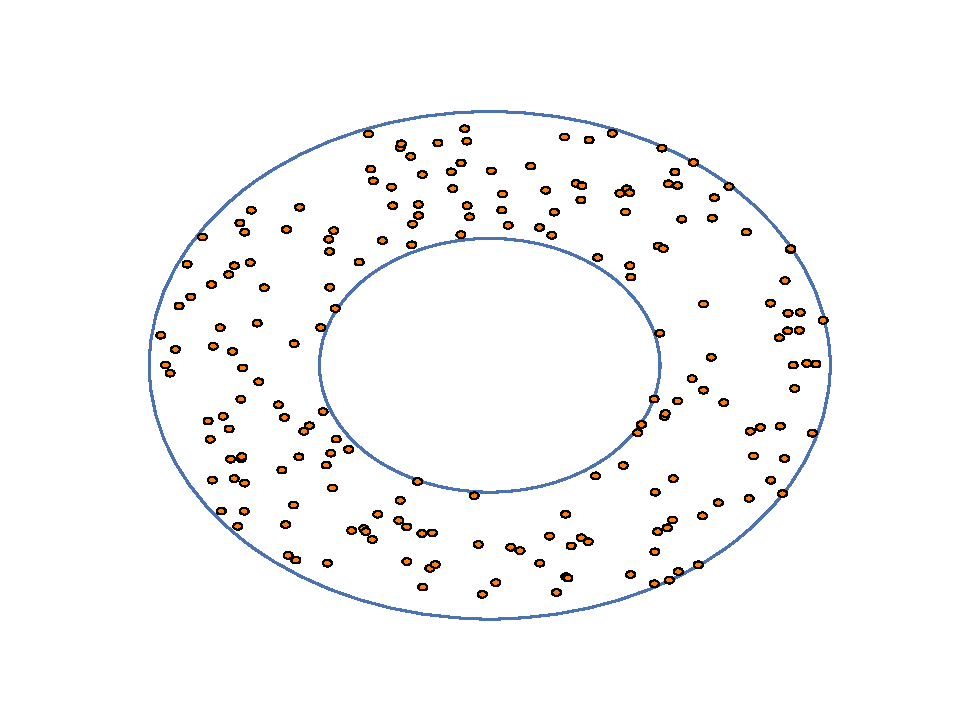
\includegraphics[scale=.5]{annulus.pdf}
    \caption{\label{annulus:points}}
 \end{subfigure}%
  \begin{subfigure}[t]{.5\linewidth}
    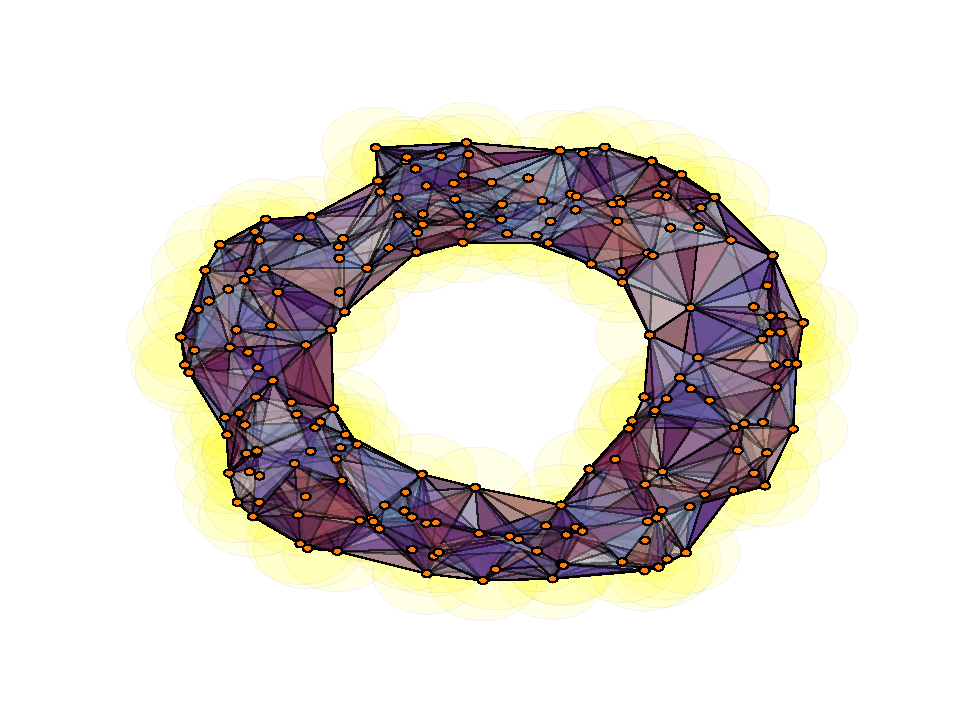
\includegraphics[scale=.5]{annulus_rips.pdf}
    \caption{\label{annulus:imposed}}
 \end{subfigure}
  \caption{\label{annulus} Imposing a simplicial complex \textbf{(b)} on data sampled from an annulus \textbf{(a)}.}
\end{figure}


If we know our space is an annulus we know what the homology is of this space, it contains a single cycle, but with raw data (figure without annulus) this can be harder to tell. This is where persistent homology comes in, a way of gaining information about the homological structure of the data space.

The basic idea is quite simple. Using the theory of simplicial homology we can impose an abstract simplicial complex on our dataset as in Figure \ref{annulus:imposed}. A natural way of doing this is defining some form of metric on our space, not necessarily metric in the sense of a metric space, such that when points are sufficiently close to each other we say they belong to the same simplex.

However, there is a problem with the idea in its naive form. How large is ``sufficiently close''? If we use too large of a distance we end up with all points in a single simplex and retrieve no valuable homological information. On the other hand, if the distance is too small we end up with a simplicial complex with very few connections between vertices and this too could prove uninformative. Persistent homology addresses this by simply considering \textit{all} of them and encoding the lifetime of homological features occuring in something called a \textit{barcode diagram}.

% First we need to recall the definition of a homotopy. A homotopy between to continuous maps $f,g$ is another continous map $H: X \times [0,1] \to Y$ such that $H(-,0) = f$ and $H(-,1) = g$. This defines an equivalence relation and we say that $f \simeq g$ meaning that $f$ is homotopy equivalent to $g$.

% We say two topological spaces $X,Y$ are homotopy equivalent, and hence overloading the meaning of this expression, when there exists continuous maps $f: X \to Y$ and $g: Y \to X$ such that $g \circ f \simeq id_{X}$  and $f \circ g \simeq id_{Y}$. This gives an equivalence relation on topological spaces and we write $X \simeq Y$ to mean that they have the same homotopy type.

% After this brief detour we can now look at nerves. We define the nerve of a finite collection of sets to be
% \[nrv(K) = \{ X \subseteq K \mid \bigcap X \neq \emptyset \}\]

% Nerve theorem. Let $F$ be a finite collection of closed convex sets in Euclidean space. Then the nerve of F and the union of the sets in F have the same homotopy type.

\section{Views}
The perhaps most natural way to impose an abstract simplicial complex on a set of points is the Cech complex
\begin{definition}[Cech complex]
For a given selection of points $\{x_{\alpha}\}$ in some Euclidean space $\mathbb{R}^{n}$ the Cech complex $C_{\epsilon}$ is given by the abstract simplicial complex whose $k$-simplices are given by $k+1$ points in the collection of points whose closed balls of radius $\epsilon/2$ have a point in common.
\end{definition}

The Cech complex is a special case of something called the nerve of a topological space. Through the Nerve theorem (cite) this guarantees that the Cech complex has the same homotopy type as the underlying space given some assumptions (what are they?). A well known result in algebraic topology is that if two spaces have the same homotopy type, they in particular have the same homology groups (really? cite, not sure about this).

However, the Cech complex is for practical purposes not feasible to compute (cite). The reason being that we need to keep the entire simplicial complex in memory and this can be quite expensive (elaborate this).

A sort of compromise is the Vietoris-Rips complex as seen in Figure \ref{manyrips}. This complex is a simplification where we do not look for points in common, but rather say that if the closed nbh around $k+1$ vertices intersect they form a $k$-simplex.

\begin{figure}
  \centering
  \begin{subfigure}[t]{.5\linewidth}
    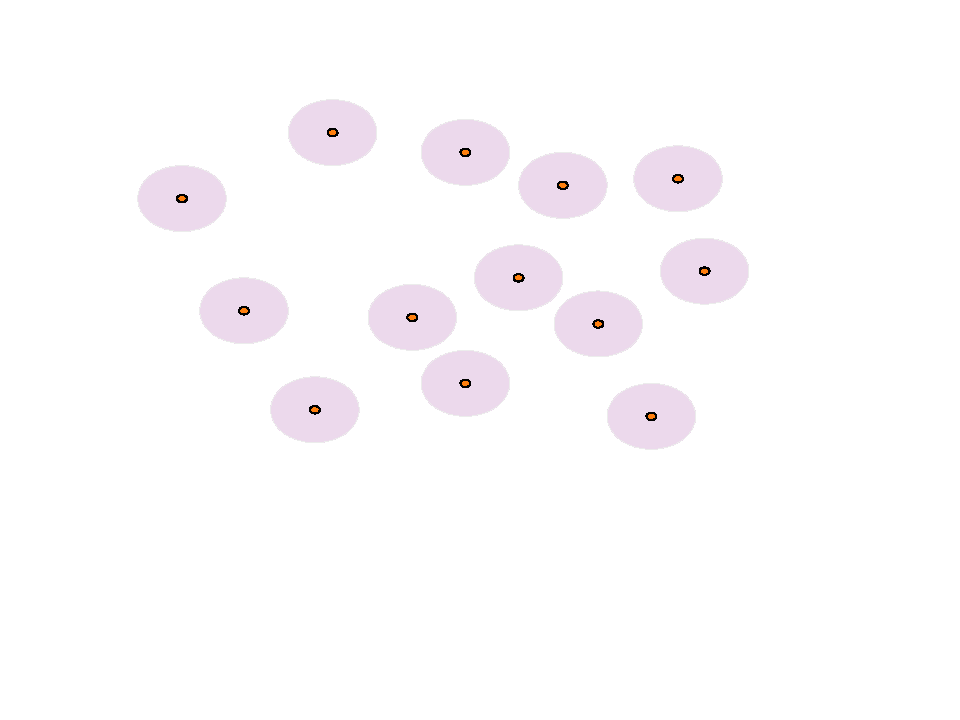
\includegraphics[scale=.5]{rips_eps=01.pdf}
    \caption{$\epsilon=0.1$}
 \end{subfigure}%
  \begin{subfigure}[t]{.5\linewidth}
    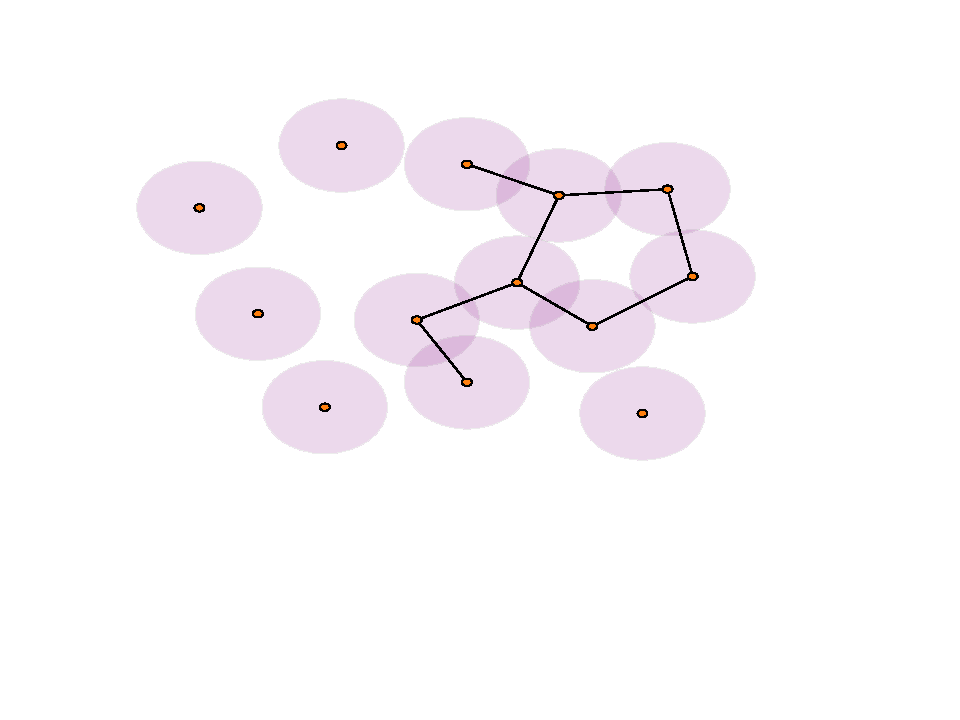
\includegraphics[scale=.5]{rips_eps=015.pdf}
    \caption{$\epsilon=0.15$}
 \end{subfigure}
  \begin{subfigure}[b]{.49\linewidth}
    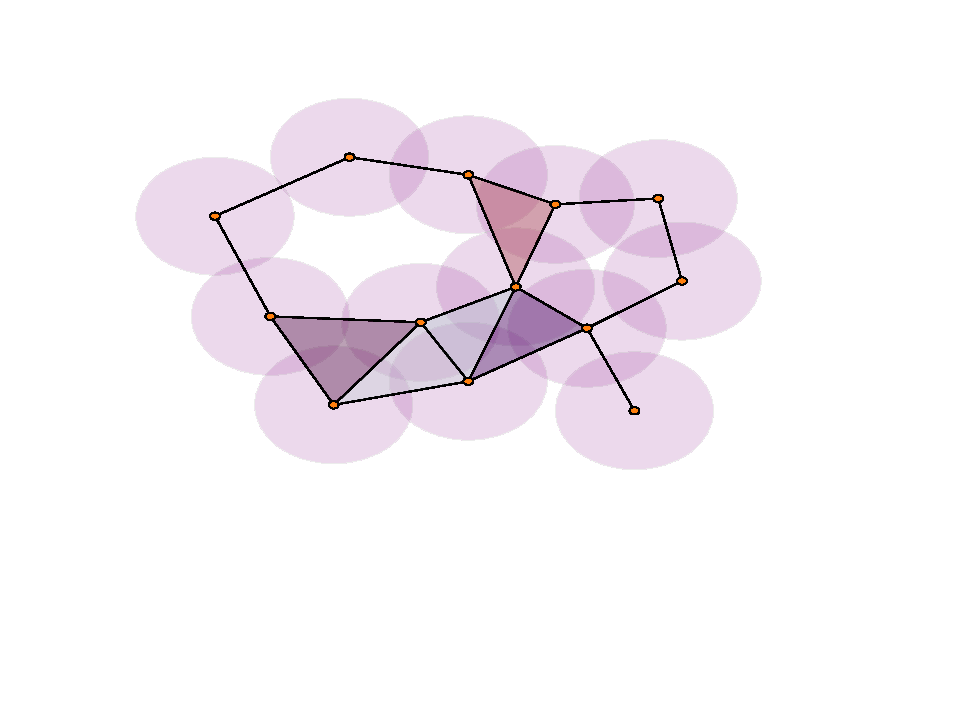
\includegraphics[scale=.5]{rips_eps=02.pdf}
    \caption{$\epsilon=0.2$}
 \end{subfigure}
  \begin{subfigure}[b]{.5\linewidth}
    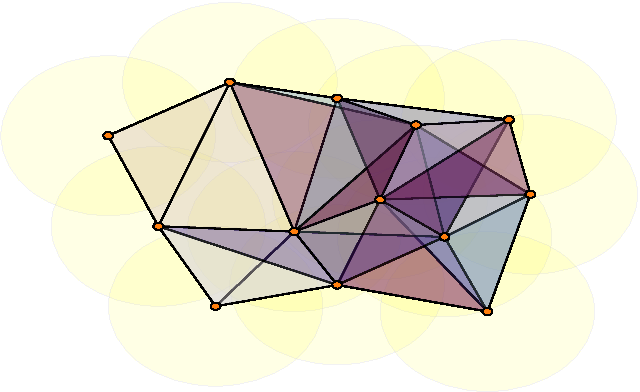
\includegraphics[scale=.5]{rips_eps=03.pdf}
    \caption{$\epsilon=0.3$}
 \end{subfigure}
 \caption{The Vietoris-Rips complex at different $\epsilon$-values.}
 \label{manyrips}
\end{figure}
\begin{definition}[Vietoris-Rips complex]
For a given selection of points $\{x_{\alpha}\}$ in some Euclidean space $\mathbb{R}^{n}$ the Vietoris-Rips complex $R_{\epsilon}$ is the abstract simplicial complex whose $k$-simplices are given by $k+1$ points which are pairwise at most $\epsilon$ apart.
\end{definition}

The Vietoris-Rips complex does not come with the same guarantee if fidelity to the underlying space as the Cech complex does. However, it is entirely defined by the vertices and the edges of the simplicial complex, allowing it to be stored as a simple graph (elaborate why the edges and vertices are enough).

Given a monotonically increasing sequence of resolutions $(\epsilon_{i})_{i \in I}$ we can associate to a finite set of points $X$ the Vietoris-Rips complexes $(R_i)_{{i \in I}}$. Then there are natural inclusions:
\begin{center}
\begin{tikzcd}
R_1 \arrow[hookrightarrow]{r}{x} & R_2 \arrow[hookrightarrow]{r}{x} & \dots \arrow[hookrightarrow]{r}{x} & R_{n-1} \arrow[hookrightarrow]{r}{x} & R_n
\end{tikzcd}
\end{center}
We then look at the image of the induced inclusions $x: H_{*}(R_{i}) \to H_{*}R_{j}$ where $i < j$. These inclusions tell us what homological features persist going from resolution $\epsilon_{i}$ to resolution $\epsilon_{j}$.

This lends some credibility to the Vietoris-Rips construction as an approximation of the underlying space since it establishes a relationship between it and the Cech complex through a result due to de Silva (cite).
\begin{lemma}
  Given $\epsilon > 0$ there is a chain of inclusions
  \[R_{\epsilon} \hookrightarrow C_{\epsilon \sqrt{2}} \hookrightarrow R_{\epsilon \sqrt{2}}\]
\end{lemma}
This tells us that any feature preserved in the inclusion $R_{\epsilon} \to R_{\epsilon \sqrt{2}}$ is also present in the Cech complex at resolution $\epsilon \sqrt{2}$ and so in the underlying topological space by theorem ?. In fact, any feature that is preserved up to resolution $\epsilon'\geq \epsilon \sqrt{2}$ is present in the Cech complex at resolution $\epsilon'$.
We are now ready to state what persistent homology formally is.
\begin{definition}
Given a persistent complex, a sequence of chain complexes with chain maps from $x: C_{*}^{i} \to C_{*}^{{i+1}}$ we define the $(i,j)$-persistent homology $H_{*}^{{i\to j}}(C)$, where $i < j$, to be the image of the induced homomorphism on homology $x_{*}: H_{*}(C_{*}^{i}) \to H_{*}(C_{*}^{j})$.
\end{definition}

In the case of the obvious filtrations created for Rips or Cech complexes $x$ will be the homomorphism induced by inclusion, but the definition is general enough that this is not necessarily the case.

\begin{definition}
The persistent Betti numbers are given by the ranks of the abelian groups $H_{*}^{i,j}$, in other words the number of generators of $H_{k}^{{i,j}}$ for all $k$ and for all $i < j$.
\end{definition}

\begin{definition}
  Let $R$ be a ring. We say $R$ is a \textbf{graded ring} if it can be decomposed as
  \[ R = \bigoplus_{i} R_{i}\]
\end{definition}
Note that given a ring $R$ the polynomial ring $R[x]$ is always a graded ring, since it can be decomposed into $R[x] = Rx^{0} \oplus Rx^{1} \oplus \dots$
\begin{definition}
  Let $R = \bigoplus_{{i}} R_{i}$ be a graded ring and $M$ a left $R-module$. We say that $M$ is a \textbf{graded $R$-module} if
  \[M = \bigoplus_{i} M_{i} \]
  where $M_{i}$ are abelian subgroups of $M$, such that $R_{i}M_{j} \subseteq M_{i+j}$.
\end{definition}
We can now see that a persistent chain complex $C_{*}$ with coefficients in a ring $R$ can be given a graded module structure by considering the graded ring $R[x]$ where $x$ are the chain maps associated with the persistent chain complex. The monomial $x^{k} \in R[x]$ sends $C_{*}^{{i}}$ to $C_{*}^{{i+k}}$ by $k$ repeated applications of $x: C_{*}^{{i}} \to C_{*}^{{i+1}}$ and so we get $Rx^{k}C^{i}_{*} \subseteq C^{{i+k}}_{*}$.

Now taking the homology $H_{*}(C)$ we retain this graded module structure, but it is not necessarily free. However, if we take our coefficient ring $R$ to be a field $\mathbb{F}$ then the Structure Theorem for PIDs (cite) gives us the following result:
\begin{theorem}
  For a finite persistence module $C$ with coefficients in a field $\mathbb{F}$,
  \[H_{*}(C;\mathbb{F}) \cong \bigoplus_{i} x^{t_{i}} \cdot \mathbb{F}[x] \oplus (\bigoplus_{j} x^{r_{j}} \cdot (\mathbb{F}[x]/(x^{s_{j}} \cdot \mathbb{F}[x]))) \]
\end{theorem}
This theorem in the case of persistence modules has quite an intuitive intepretation. The free part consists of features which appear at resolution indexed by $t_{i}$ and continue to exist for all future resolutions. The torsion part consists of the features which appear at resolution indexed by $r_{j}$ and disappear at resolution $r_{j}+s_{j}$.

While the restriction to a field $\mathbb{F}$ somewhat limits the usefulness of persistence homology, often in practice we prefer working in $\mathbb{Z}_{2}$ due to computational aspects and hence it poses no real problem.
\section{Barcodes}
With our algebraic description (in ref theorem above) of persistence we are now able to state the first invariant of persistent homology. This invariant is known as a \textbf{barcode}.

This is a visual depiction of $H_{*}(C; \mathbb{F})$ where each bar depicts the birth and death of a particular generator in one of the homology groups.

\begin{theorem}
  The rank of the persistent homology group $H^{{i \to j}}_{k}(C;\mathbb{F})$ is equal to the number of intervals in the barcode of $H_{k}(C;\mathbb{F})$ in the interval of parameters $[i,j]$.
  \end{theorem}
  \begin{proof}
  (TODO: Show this not very difficult proof)
  \end{proof}
  (TODO: Add a remark here explaining why this is interesting.)

  Example. In Figure \ref{annulus_barcode} we see a barcode generated from points sampled from an annulus. Note that for small values of $\epsilon$ there are many generators of $H_{0}$, this is because the vertices have not been connected into a single component yet. We see that there some short intervals appearing for $H_{1}$ at around $\epsilon=0.3$ and we can see that these are not the hole that would represent the annulus, but rather noise that appears before $\epsilon$ has become large enough. But we see at around $\epsilon=0.6$ that the simplicial complex now captures the shape of the annulus and indeed the barcode reports that we have one generator of $H_{0}$, the only connected component, and one generator of $H_{1}$ which is the hole in the middle of the annulus. We see that this hole in the middle of the annulus is gone when $\epsilon=1$ which highlights that it is difficult to find an optimal $\epsilon$.

\begin{figure}
  \centering
\begin{tikzpicture}
\node[inner sep=0pt] (barcode) at (0,0)
    {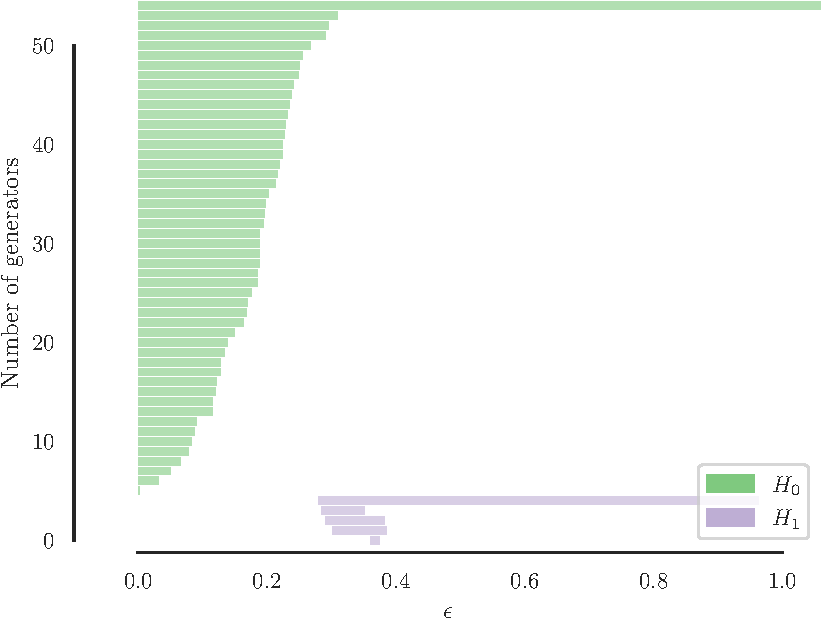
\includegraphics[scale=0.7]{barcode.pdf}};

\node[draw=black!100,line width=0.6mm, inner sep=0pt] (annulus0) at (-3.2,5.1)
    {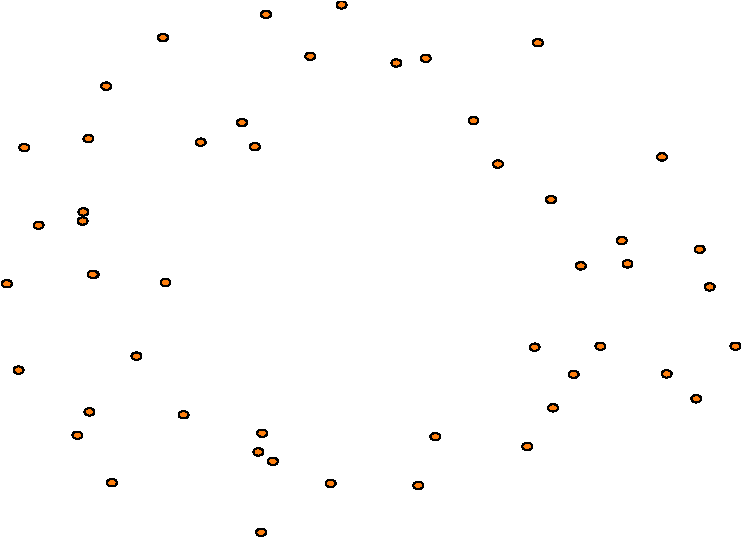
\includegraphics[scale=0.3]{annulus_eps0.pdf}};
    \draw[dotted,thick] (annulus0.south) -- (-3.2,-2.9);

\node[draw=black!100,line width=0.6mm, inner sep=0pt] (annulus3) at (-1,8)
    {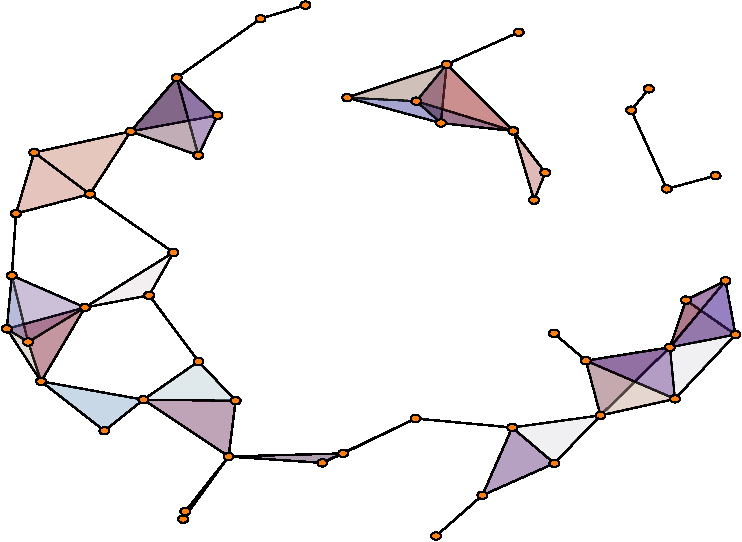
\includegraphics[scale=0.3]{annulus_eps3.pdf}};
\draw[dotted,thick] (annulus3.south) -- (-1,-2.9);

\node[draw=black!100,line width=0.6mm, inner sep=0pt] (annulus5) at (1.2,5.1)
    {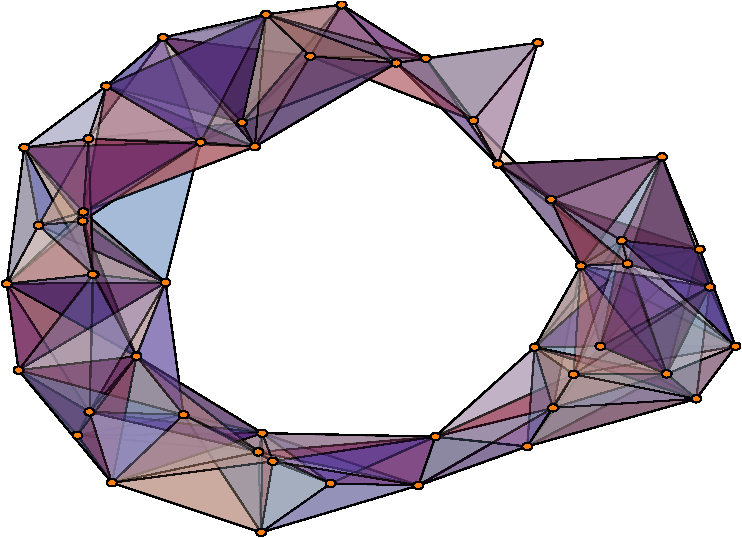
\includegraphics[scale=0.3]{annulus_eps5.pdf}};
    \draw[dotted,thick] (annulus5.south) -- (1.2,-2.9);
\node[draw=black!100,line width=0.6mm, inner sep=0pt] (annulus10) at (4.4,8)
    {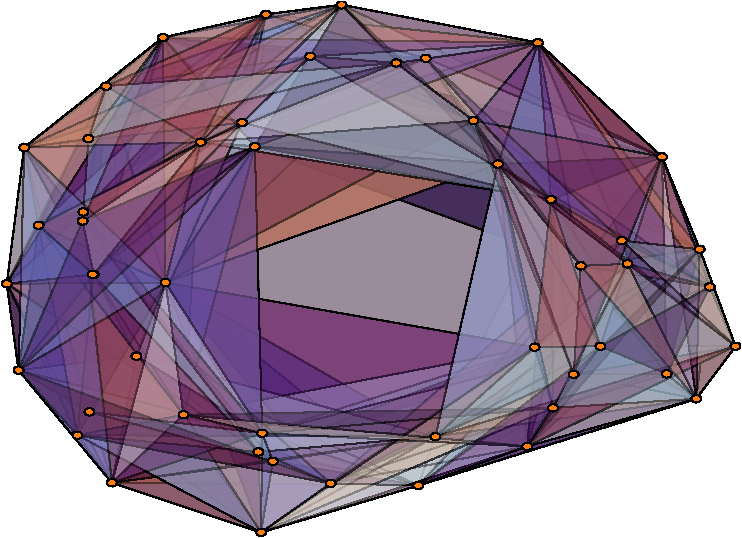
\includegraphics[scale=0.3]{annulus_eps10.pdf}};
\draw[dotted,thick] (annulus10.south) -- (4.4,-1.8);
\draw[dotted,thick] (4.4,-2.74) -- (4.4,-2.9);
\end{tikzpicture}
\caption{\label{annulus_barcode} Persistence barcode showing the birth and death of generators in the homology groups of a Vietoris-Rips complex approximated from points sampled from an annulus at different $\epsilon$. }
\end{figure}
  \section{Persistence Diagrams}
  Another way of illustrating is the persistence diagram which consists of..
  \section{Metrics}
  If we compute two barcodes, how do we compare them? There are two suitable metrics for this.. Wasserstein and Bottleneck.
\section{Computation of }
Some aspects of the computational part of this. How is it done in practice? Mention an example but do not dwell too much on this. Perhaps go into smith normal form and how it all translates to linear algebra?
%%% Local Variables:
%%% mode: latex
%%% TeX-master: "thesis.tex"
%%% End:
